\documentclass[11pt,letterpaper]{article}
\usepackage[margin=0.85in,headheight=14pt]{geometry}
\usepackage[T1]{fontenc}
\usepackage{lmodern}
\usepackage{amsmath,amssymb,graphicx,booktabs}
\usepackage[font=small,labelfont=bf]{caption}
\usepackage{fancyhdr}
\usepackage[hidelinks]{hyperref}
\pagestyle{fancy}
\fancyhf{}
\fancyhead[L]{\small PHYSICS 5409: Computational Physics Lab}
\fancyhead[R]{\small Jeremiah Bender}
\fancyfoot[C]{\thepage}
\setlength{\parindent}{1.2em}
\setlength{\parskip}{3pt}
\setlength{\textfloatsep}{10pt}
\setlength{\intextsep}{9pt}
\newcommand{\avg}[1]{\left\langle #1\right\rangle}
\newcommand{\BN}{B_{\mathrm N}}
\newcommand{\chiabs}{\chi_{|m|}}
\graphicspath{{images/}}
\hypersetup{pdftitle={Critical behavior of the clean three-dimensional lattice phi4 model: progress report},pdfauthor={Jeremiah Bender}}
\begin{document}
\begin{center}
{\Large\bfseries Critical Behavior of the Clean\\[2pt]
Three-Dimensional Lattice \(\boldsymbol{\phi^4}\) Model}\\[6pt]
{\large Midsemester Progress Report}\\[4pt]
Jeremiah Bender \quad $\cdot$ \quad October 30, 2026
\end{center}
\vspace{-8pt}

\section{Refined goals and background}
I am using the three-dimensional lattice $\phi^4$ model to study how an
ordered state develops as temperature decreases. Each site has a real-valued
field, and neighboring fields favor alignment. With one scalar order
parameter, sign-reversal symmetry, and short-range interactions, I expect
a continuous transition to fall in the three-dimensional Ising universality class.

My goal is to estimate $T_c$ and the exponents $\nu$, $\beta$, and $\gamma$
from several lattice sizes. These describe the correlation length, order
parameter, and susceptibility near the transition. The current results use
a fully occupied lattice with fixed couplings. I also want to explore how
random vacancies affect the transition and why quenched disorder can lead
to a different universality class.

One physical example is the Ising antiferromagnet FeF$_2$, where the field
can represent staggered magnetization, the difference
between the magnetizations of the two sublattices~\cite{belanger}.
In a binary liquid near demixing, it can represent the local composition
relative to the critical composition. Experiments on water--2,6-lutidine
show how these fluctuations produce critical Casimir forces between a
colloid and a surface~\cite{gambassi}. Calculating those forces would
require adding surfaces and their boundary conditions to this bulk model.

Since the proposal, I have implemented Metropolis sampling and parallel
tempering and completed the first exponent fits. I will use these clean
results as a reference when I add vacancies. The simulation and analysis
code are in the project repository~\cite{repository}.

\section{Implemented methods}
\subsection{Hamiltonian and local Metropolis updates}
The simulation uses a periodic simple cubic lattice with $N=L^3$ sites and
a real field $\phi_i$ at each site. The Hamiltonian is
\begin{equation}
H=-J\sum_{\langle ij\rangle}\phi_i\phi_j+
 \sum_i\left(\frac r2\phi_i^2+\frac u4\phi_i^4\right),
\qquad J=1,\quad r=-1,\quad u=1,
\label{eq:H}
\end{equation}
where each nearest-neighbor bond is counted once. I set $k_{\mathrm B}=1$,
so a configuration has weight proportional to $\exp(-H/T)$.

One sweep visits each site and proposes
$\phi_i'=\phi_i+\delta$, with $\delta$ drawn uniformly from a fixed symmetric
interval. If $S_i$ is the sum of the six neighboring fields, the energy
change is
\begin{equation}
\Delta H=-J(\phi_i'-\phi_i)S_i+
 \frac r2(\phi_i'^2-\phi_i^2)+\frac u4(\phi_i'^4-\phi_i^4).
\end{equation}
The proposal is accepted with probability
$\min[1,\exp(-\Delta H/T)]$~\cite{metropolis}.
I use both random and ordered starting fields. The proposal width is
adjusted during the initial sweeps and held fixed afterward. I checked
the local energy change against full-energy calculations and analytic
identities.

\newpage
\subsection{Parallel tempering}
Near the transition, large regions fluctuate together, and local updates
change these regions slowly. I use parallel tempering so configurations
can visit higher temperatures, where ordered regions break up and
reorganize, before returning near $T_c$~\cite{earl}. These visits can
help reduce correlations between measurements. How well this works
depends on the local Metropolis updates and how long replicas spend
at the other temperatures; slow fluctuations can still remain.

Replicas run at different temperatures and attempt exchanges between
neighboring pairs, alternating even and odd pairs. For total energies
$H_a,H_b$ at $T_a<T_b$, the exchange probability is
\begin{equation}
P_{\mathrm{swap}}=\min\!\left\{1,
 \exp\left[\left(\frac{1}{T_a}-\frac{1}{T_b}\right)(H_a-H_b)\right]\right\}.
\end{equation}
I group measurements by temperature after exchanges. The main runs use
$L=16,24,32,48$, with 17, 25, 25, and 40 temperatures spanning
$14.9$--$16.5$. For each size, I ran two independent temperature ladders:
one from random fields and one from an ordered state, using separate
random-number streams. Every temperature has 2,000 adaptation sweeps,
50,000 settling sweeps, and 500,000 measurement sweeps. Exchanges and saved
measurements occur every five sweeps.

\subsection{Observables and statistical errors}
For each configuration, $e=H/N$ and $m=N^{-1}\sum_i\phi_i$. I calculate
\begin{equation}
 B_4=\frac{\avg{m^4}}{\avg{m^2}^2},\qquad
 \BN=\frac{3-B_4}{2},\qquad
 \chiabs=\frac NT\left(\avg{m^2}-\avg{|m|}^2\right).
\end{equation}
The order parameter is $\avg{|m|}$. The normalized Binder cumulant
approaches one in the ordered limit and zero in the Gaussian limit.

I calculate autocorrelation separately for energy, $|m|$, $m^2$, and
$m^4$ at each temperature and lattice size. For a history $x_1,\ldots,x_n$,
I subtract its mean $\bar x$ and multiply pairs of deviations separated
by $k$ saved measurements. Averaging these products gives
\begin{equation}
 C_x(k)=\frac{1}{n-k}\sum_{i=1}^{n-k}(x_i-\bar x)(x_{i+k}-\bar x),
 \qquad \rho_x(k)=\frac{C_x(k)}{C_x(0)}.
\end{equation}
If measurements tend to stay on the same side of the mean, their products
are positive. As this memory fades, $\rho_x(k)$ approaches zero.
The normalization gives $\rho_x(0)=1$. I estimate the integrated
correlation time by adding the correlations over a range of time gaps:
\begin{equation}
 \tau_{\mathrm{int},x}=\frac12+\sum_{k=1}^{W}\rho_x(k),
 \qquad n_{\mathrm{eff}}\simeq\frac{n}{2\tau_{\mathrm{int},x}}.
\end{equation}
The upper limit $W$ keeps noisy estimates at large time gaps from
dominating the sum. The correlation time is measured in saved-measurement
units; each saved measurement is five sweeps apart. Here $n$ is the total
number of saved measurements, and $n_{\mathrm{eff}}$ is the estimated
number of independent measurements that would give similar precision.
Positive correlations reduce this effective count. This estimate assumes
equilibrium and can miss weak, slow fluctuations. I also increase the
block length to check whether the error estimates level off.

Point error bars come from leaving out one time block at a time and
recalculating the observable (block jackknife). Central fits use 2,000
saved samples per block, and plotted error bars use 5,000.

\newpage
\section{Finite-size scaling and preliminary results}
Near $T_c$, the correlation length becomes comparable to the lattice
size. Observables at the transition then scale with $L$~\cite{fisher}:
\begin{equation}
 \left|\frac{dB_4}{dT}\right|\propto L^{1/\nu},\qquad
 \avg{|m|}\propto L^{-\beta/\nu},\qquad
 \chiabs\propto L^{\gamma/\nu}.
\end{equation}
I fit quadratic temperature curves over $15.30\leq T\leq15.34$ and find
the $L=24,48$ Binder crossing at $T_c\simeq15.3101$. Weighted log--log
fits at this temperature give powers $1/\nu=1.640$, $-\beta/\nu=-0.519$,
and $\gamma/\nu=1.957$ (Figure~\ref{fig:scaling}).

For uncertainty, I resample time blocks with replacement and repeat the
crossing and both fitting stages 2,000 times. Each ladder uses the same
selected blocks across all temperatures and moments. The two independent
ladders are resampled separately, then combined with their original sample
weights. Point-error weights stay fixed. Table~\ref{tab:exponents} gives
the middle 95\% of the resulting $T_c$ and exponent estimates.

\begin{figure}[ht]
\centering
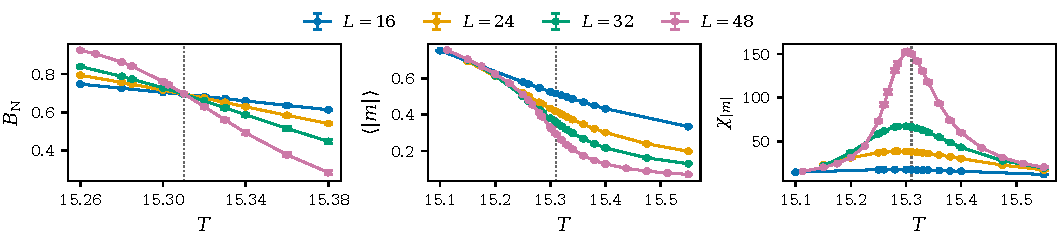
\includegraphics[width=\linewidth]{transition-curves.pdf}
\caption{Binder crossing, magnetization, and susceptibility for
$L=16,24,32,48$. Error bars are one block-jackknife standard error using
25,000-sweep blocks. The dotted line marks the fitted crossing temperature.}
\label{fig:curves}
\end{figure}

\begin{figure}[ht]
\centering
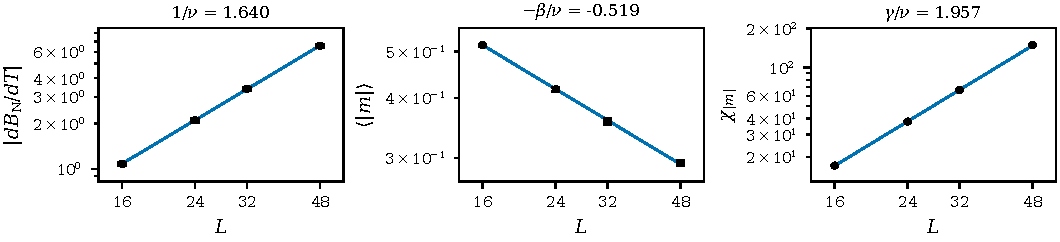
\includegraphics[width=\linewidth]{scaling-fits.pdf}
\caption{Size scaling at $T_c\simeq15.3101$, on logarithmic axes.
Points are interpolated values; lines are the weighted power-law fits.
The slopes give $1/\nu$, $-\beta/\nu$, and $\gamma/\nu$.
Error bars are one bootstrap standard error, including uncertainty in $T_c$.}
\label{fig:scaling}
\end{figure}

\begin{table}[ht]
\centering
\caption{Effective finite-size estimates and marginal 95\% statistical
intervals. The Ising comparison uses Ref.~\cite{hasenbusch}; $\beta$ and
$\gamma$ are derived from its $\nu$ and $\eta$.}
\small
\begin{tabular}{lrrr}
\toprule
Quantity & Estimate & 95\% interval & 3D Ising comparison\\
\midrule
$T_c$ & 15.3101 & [15.3069, 15.3137] & model dependent\\
$\nu$ & 0.610 & [0.580, 0.639] & 0.63002\\
$\beta$ & 0.316 & [0.292, 0.342] & 0.32644\\
$\gamma$ & 1.193 & [1.141, 1.243] & 1.23719\\
\bottomrule
\end{tabular}
\label{tab:exponents}
\end{table}

The susceptibility peak rises from 17.45 at $L=16$ to 152.93 at $L=48$.
All three exponent intervals include the literature values; longer runs
and larger lattices are needed to check the remaining shifts.

\newpage
\section{Difficulties and solutions}
\subsection{Slow fluctuations and finite histories}
The first short runs had broad susceptibility peaks and strongly
correlated measurements. The peak became clearer at larger sizes.
Some replicas still move slowly through the temperature ladder: three
in the $L=48$ runs made no full round trip. Errors for some observables grow by
20--30\% when block length increases from 1,000 to 5,000 saved samples.
The longer choice leaves only 20 blocks per ladder, so I need longer
histories to check where the errors level off.

\subsection{How the fitting choices affect the exponents}
For the main estimate, I fit temperatures from $15.30$ to $15.34$.
Widening this to $15.28$--$15.36$ shifts $\nu$ to about 0.654. Over the
wider range, a quadratic fits the $L=48$ susceptibility poorly: the
residuals are large compared with the point errors. Figure~\ref{fig:sensitivity}
shows this result in red. I have kept it in the comparison because the
shift is larger than those from the other fitting choices.

The other rows change the block length, use a linear temperature fit,
remove $L=16$, change the Binder crossing pair, or fit each initial-state
run separately. These changes produce smaller shifts. Removing $L=16$
checks the influence of small lattices, and fitting each start separately
checks whether the two runs give consistent estimates. Longer runs and
larger sizes should make these comparisons more informative.

\begin{figure}[ht]
\centering
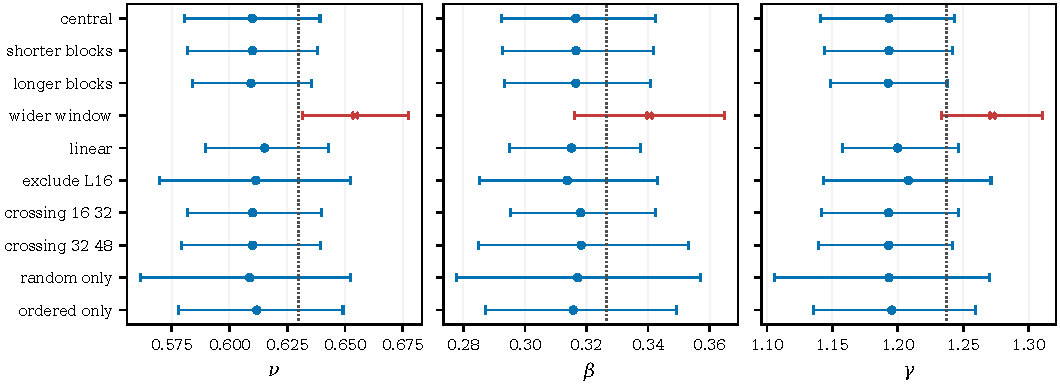
\includegraphics[width=\linewidth]{exponent-sensitivity.pdf}
\caption{Each row changes one analysis choice. Bars are 95\% statistical
intervals; dotted lines are the Ising reference. The red wider-window
result has a poor local quadratic fit.}
\label{fig:sensitivity}
\end{figure}

\paragraph{Hyperscaling as a consistency check.}
For a scale-invariant critical magnetization distribution, both
$\avg{m^2}$ and $\avg{|m|}^2$ scale as $L^{-2\beta/\nu}$.
The susceptibility definition then gives
$\chiabs\propto L^{d-2\beta/\nu}$. Comparing this with
$L^{\gamma/\nu}$ gives the hyperscaling relation
\begin{equation}
 \frac{2\beta}{\nu}+\frac{\gamma}{\nu}=d=3.
\end{equation}
The fitted combination is 2.994, with a 95\% interval of [2.954,3.038].
The powers are fitted independently before making this comparison.

\newpage
\section{Plan for completion and quenched disorder}
\paragraph{Finish the clean calculation.}
I will extend the $L=32,48$ runs to check block-error stability and add a
full temperature ladder at $L=64$. Repeating the fits across windows and
sets of sizes will help separate interpolation effects from finite-size
corrections. Comparisons of independent starts and production halves
will continue to check the sampling.

\paragraph{Explore why disorder can change universality.}
I would like to randomly remove a small fraction of sites, keep that
vacancy pattern fixed throughout each simulation, and repeat the calculation
for several patterns. This is quenched disorder: the fields fluctuate,
while the vacancies stay fixed. A small comparison could show how
vacancies change the ordering curves, susceptibility peak, and transition
temperature. Differences between vacancy patterns must be averaged as
well as the thermal fluctuations within each pattern.

For weak, uncorrelated dilution, the Harris criterion predicts that
disorder changes the clean critical behavior when
$d\nu_{\mathrm{clean}}<2$~\cite{harris}. Here
$3(0.63002)\simeq1.89<2$, so disorder is a relevant perturbation.
Published simulations find a randomly diluted Ising universality class
with $\nu\simeq0.683$, compared with the clean value near
0.630~\cite{randomising}.

For this stage, I want to show how vacancies affect the transition and
look for changes in the size dependence. I do not expect enough time to
measure the disordered exponents precisely. A shift in $T_c$ alone would
not establish new exponents. I will compare what the runs show with the
Harris criterion and published results, and be clear about which scaling
differences the data can resolve.

\begin{thebibliography}{9}
\small
\bibitem{belanger}
D.~P.~Belanger and H.~Yoshizawa, ``Neutron scattering and the critical
behavior of the three-dimensional Ising antiferromagnet FeF$_2$,''
\emph{Phys. Rev. B} \textbf{35}, 4823--4830 (1987).
\href{https://doi.org/10.1103/PhysRevB.35.4823}{doi:10.1103/PhysRevB.35.4823}.

\bibitem{gambassi}
A.~Gambassi, A.~Maciolek, C.~Hertlein, U.~Nellen, L.~Helden,
C.~Bechinger, and S.~Dietrich, ``Critical Casimir effect in classical
binary liquid mixtures,'' \emph{Phys. Rev. E} \textbf{80}, 061143 (2009).
\href{https://arxiv.org/abs/0908.1795}{arXiv:0908.1795}.

\bibitem{metropolis}
N.~Metropolis, A.~W.~Rosenbluth, M.~N.~Rosenbluth, A.~H.~Teller, and
E.~Teller, ``Equation of State Calculations by Fast Computing Machines,''
\emph{J. Chem. Phys.} \textbf{21}, 1087--1092 (1953).
\href{https://doi.org/10.1063/1.1699114}{doi:10.1063/1.1699114}.

\bibitem{earl}
D.~J.~Earl and M.~W.~Deem, ``Parallel Tempering: Theory, Applications,
and New Perspectives'' (2005).
\href{https://arxiv.org/abs/physics/0508111}{arXiv:physics/0508111}.
\href{https://doi.org/10.1039/B509983H}{doi:10.1039/B509983H}.

\bibitem{fisher}
M.~E.~Fisher and M.~N.~Barber, ``Scaling Theory for Finite-Size Effects
in the Critical Region,'' \emph{Phys. Rev. Lett.} \textbf{28}, 1516 (1972).
\href{https://doi.org/10.1103/PhysRevLett.28.1516}{doi:10.1103/PhysRevLett.28.1516}.

\bibitem{hasenbusch}
M.~Hasenbusch, ``A Finite Size Scaling Study of Lattice Models in the
three-dimensional Ising Universality Class,''
\emph{Phys. Rev. B} \textbf{82}, 174433 (2010).
\href{https://arxiv.org/abs/1004.4486}{arXiv:1004.4486}.
\href{https://doi.org/10.1103/PhysRevB.82.174433}{doi:10.1103/PhysRevB.82.174433}.

\bibitem{harris}
A.~B.~Harris, ``Effect of random defects on the critical behaviour of
Ising models,'' \emph{J. Phys. C} \textbf{7}, 1671 (1974).
\href{https://doi.org/10.1088/0022-3719/7/9/009}{doi:10.1088/0022-3719/7/9/009}.

\bibitem{randomising}
M.~Hasenbusch, F.~Parisen Toldin, A.~Pelissetto, and E.~Vicari,
``Universality class of 3D site-diluted and bond-diluted Ising systems'' (2007).
\href{https://arxiv.org/abs/cond-mat/0611707}{arXiv:cond-mat/0611707}.

\bibitem{repository}
J.~Bender, \emph{Clean 3D phi4: Computational Physics Lab}, project repository.
\url{https://github.com/ShadowQFT/phi4}.
\end{thebibliography}
\end{document}
